\documentclass[serif,mathserif, 12pt]{beamer}
\usepackage{etex}
\usepackage{amsmath, amsfonts, epsfig, xspace}
\usepackage{algorithm,algorithmic}
\usepackage{pstricks,pst-node}
\usepackage{multimedia}
\usepackage[normal,tight,center]{subfigure}
\setlength{\subfigcapskip}{-.5em}
\usepackage{tkz-euclide}
\usetkzobj{all}
\usepackage{beamerthemesplit}
\usetheme{lankton-keynote}
\usepackage{graphicx,color}
% remove caption of figure
\usepackage[labelformat=empty]{caption}

\usepackage[none]{hyphenat} % hyphenation is ugly in slides
\usepackage{parskip}

\usepackage{relsize} % \smaller to change size

\usepackage{tikz}
\usetikzlibrary{calc}

\usetikzlibrary{arrows}

\newcommand{\TikzDraw}[2][]{
  \begin{tikzpicture}[overlay, remember picture, shift={(current page.center)}, #1]
    #2
  \end{tikzpicture}
}

\newcommand{\gridlines}{
  \TikzDraw{
    \draw[help lines,xstep=.2,ystep=.2,red!20] (current page.south west) grid (current page.north east);
    \draw[help lines,xstep=1,ystep=1,red] (current page.south west) grid (current page.north east);
    \foreach \x in {-15,-14,...,15} {
      \node [anchor=north, red] at (\x,0) {\tiny \x};
      \node [anchor=east,red] at (0,\x) {\tiny \x};
    }
  }
}

\newcommand{\DrawOnImg}[3][]
{
  \begin{tikzpicture}
    \node[anchor=south west,inner sep=0] (image) at (0,0){
      #2
    };
    \begin{scope}[x={(image.south east)},y={(image.north west)}]
      \ifthenelse{\equal{#1}{grid}}
                 {\draw[color=blue, style=dashed] (0,0) grid[xstep=.1, ystep=.1] (1.0001,1.0001);}
                 {}
                 #3
    \end{scope}
  \end{tikzpicture}
}

\usetikzlibrary{matrix}

\newcommand{\BOLD}[1]{\mathbf{#1}}
\newcommand{\BOLDG}[1]{\boldsymbol{#1}}
\newcommand{\PDIF}[2]{\frac{\partial #1}{\partial #2}}
\newcommand{\TODO}[1]{\textcolor{red}{#1}}
\newcommand{\TODOB}[1]{\textcolor{blue}{#1}}
\newcommand{\TODOG}[1]{\textcolor{green!50!black}{#1}}
\newcommand{\argmin}{\operatornamewithlimits{arg\min}}
\DeclareMathOperator{\tr}{tr}
\DeclareMathOperator{\cond}{cond}
\DeclareMathOperator{\ST}{s.t.}
\DeclareMathOperator{\diag}{diag}
\DeclareMathOperator{\Div}{div}

\title[\hspace{2em}\insertframenumber/\inserttotalframenumber]{Mechanical Characterization of Structured Sheet Materials}
\date{28th, September 2018}

\author{Disney Research}

\makeatletter
\let\@@magyar@captionfix\relax
\makeatother

\begin{document}

\maketitle

\begin{frame}
  \frametitle{M. C. Escher}
  \TikzDraw {
    \node at (-3, 0) {
      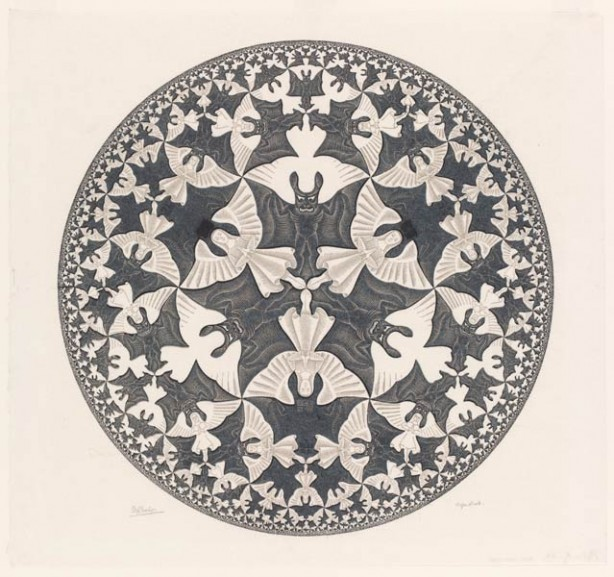
\includegraphics[width=0.5\textwidth]{img/escher-0}
    };
    \node at (3, 0) {
      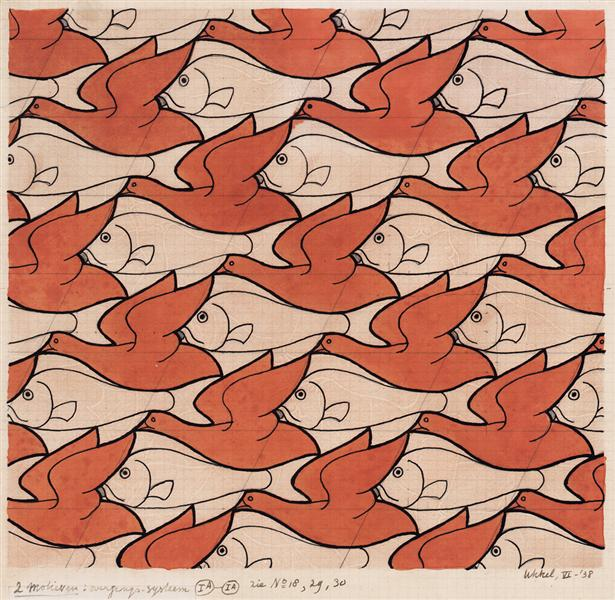
\includegraphics[width=0.48\textwidth]{img/escher-1}
    };
  }
\end{frame}

\begin{frame}
  \frametitle{Escherization}
  \TikzDraw {
    \node at (-3, 0) {
      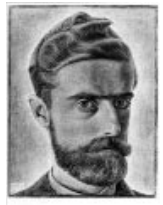
\includegraphics[width=0.3\textwidth]{img/escher}
    };
    \node at (2.5, 0) {
      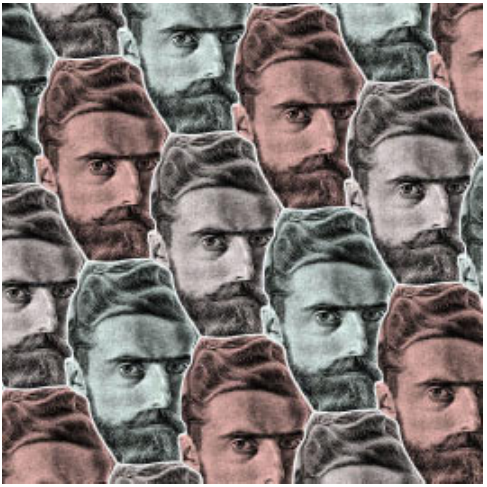
\includegraphics[width=0.5\textwidth]{img/escherization}
    };
    \node at (-3, -3) {
      [Kaplan 2000]
    };
  }
\end{frame}

\begin{frame}
  \frametitle{Tillings}
  \begin{itemize}
  \item Tilling of the plane
    \begin{itemize}
    \item[-] A collection of shapes (tiles) that cover the plane without any gaps and overlays.
    \end{itemize}
    \pause
  \item Isohedral tilling
    \begin{itemize}
    \item[-] IH1,...,IH93
    \end{itemize}
  \end{itemize}
\end{frame}

\begin{frame}
  \frametitle{Isohedral Tillings}
  \TikzDraw{
    \node at (-0.39\textwidth, 0) {
      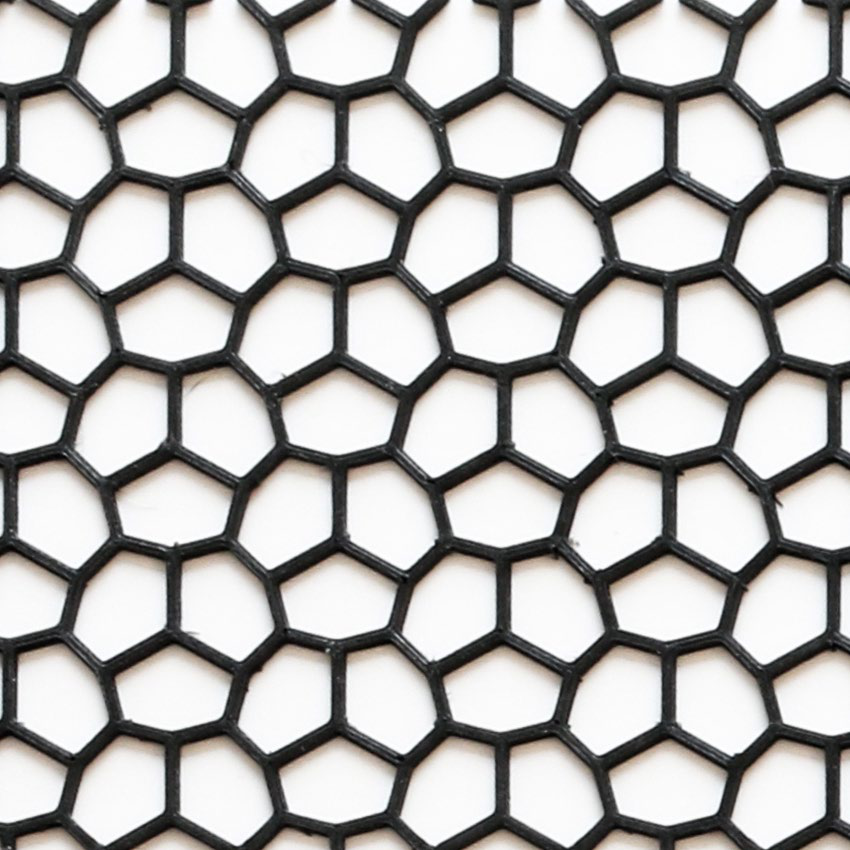
\includegraphics[width=0.25\textwidth]{img/paper-000}
    };
    \node at (-0.13\textwidth, 0) {
      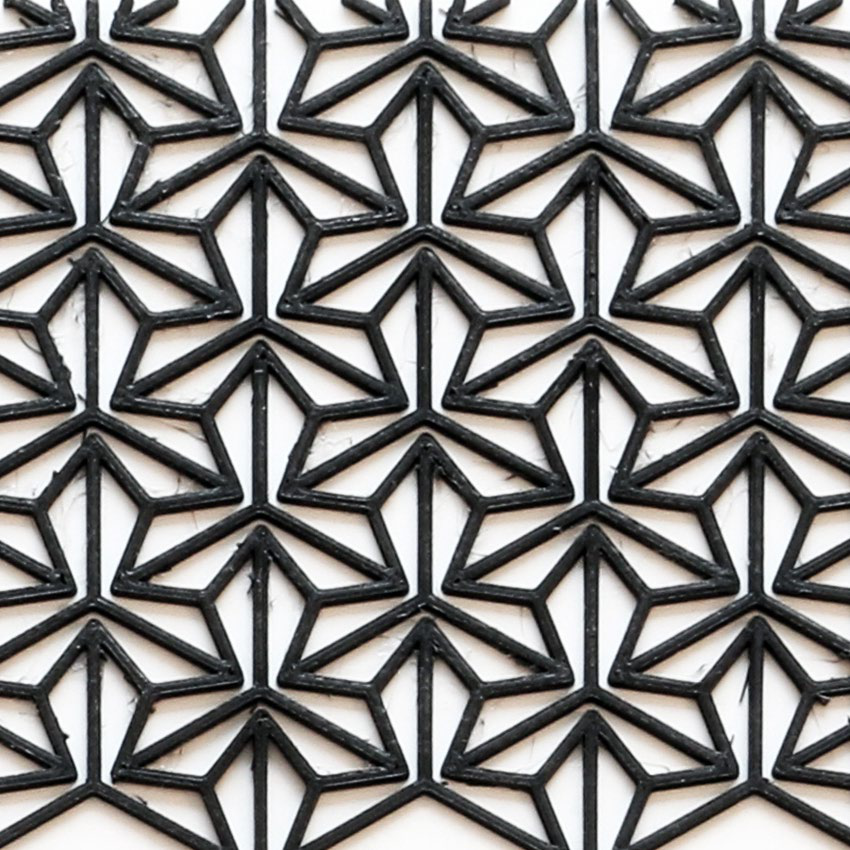
\includegraphics[width=0.25\textwidth]{img/paper-001}
    };
    \node at (0.13\textwidth, 0) {
      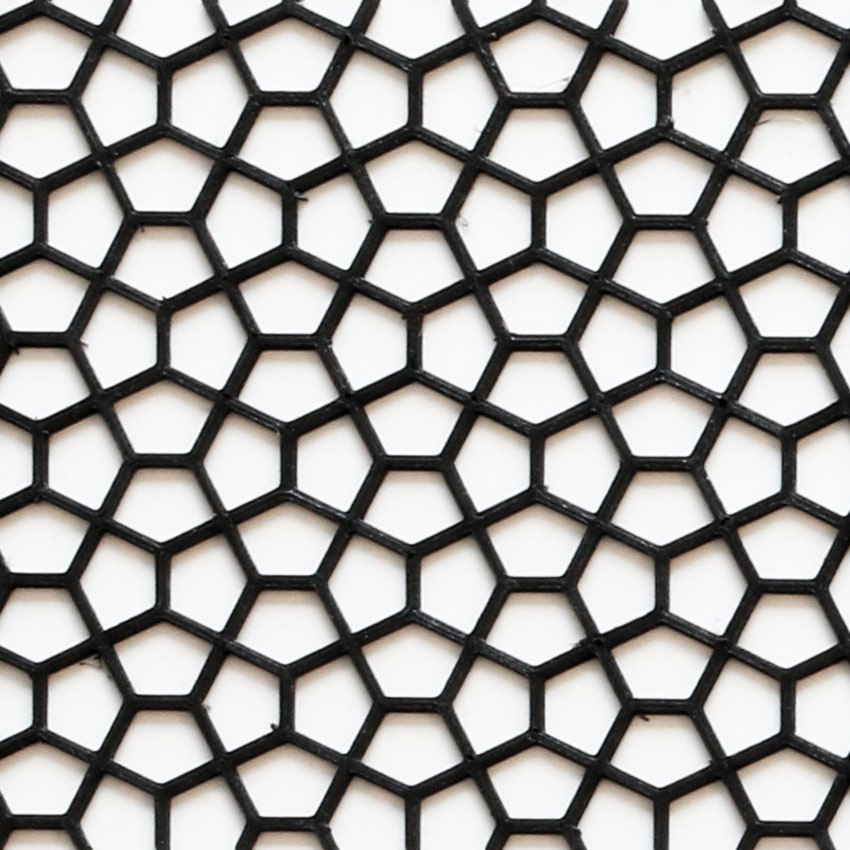
\includegraphics[width=0.25\textwidth]{img/paper-002}
    };
    \node at (0.39\textwidth, 0) {
      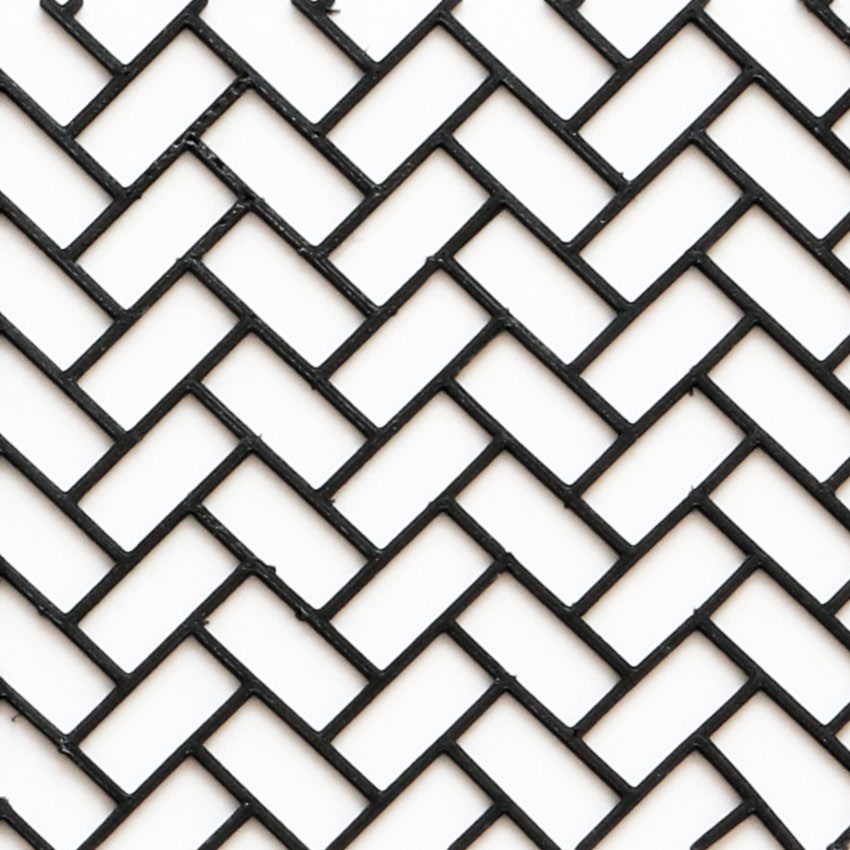
\includegraphics[width=0.25\textwidth]{img/paper-003}
    };
    \visible<2-> {
      \node at (0, 0) {
        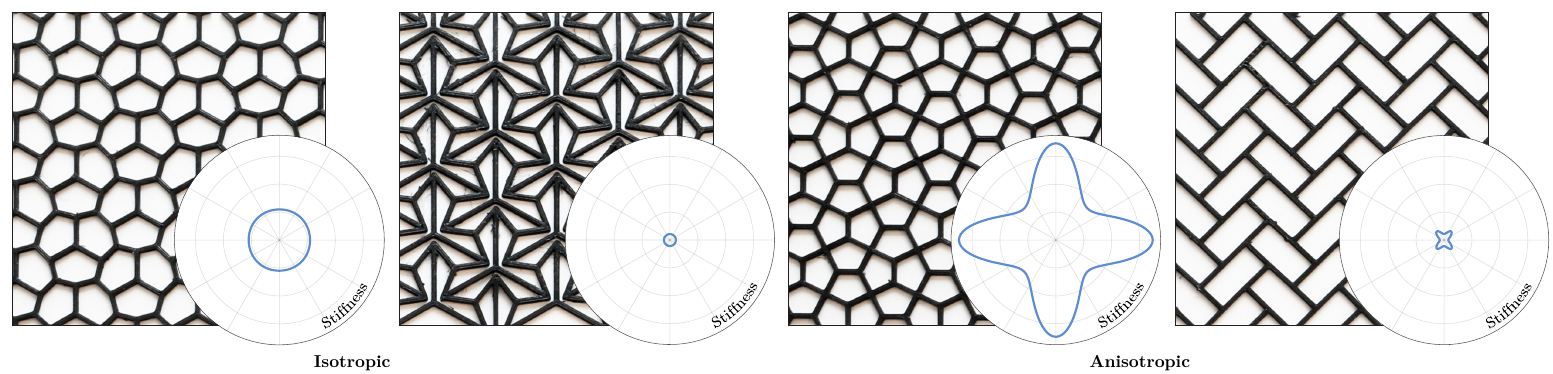
\includegraphics[width=1.1\textwidth]{img/teaser}
      };
      \node at (0, -2.5) {
        \TODO{Mechanical property?}
      };
    }
  }  
\end{frame}

\begin{frame}
  \frametitle{Overview}
  \begin{itemize}
  \item Physical modeling of sheet network
    \begin{itemize}
    \item[-] Mesoscopic model
    \item[-] Macroscopic model
    \end{itemize}
  \item Homogenization
  \item Characterization
  \end{itemize}
\end{frame}

\begin{frame}
  \frametitle{Mesoscopic Model}
  \begin{itemize}
  \item Discrete elastic rod
    \begin{itemize}
    \item[-] Stretching, bending, twisting
    \end{itemize}
  \end{itemize}
  \TikzDraw {
    \node at (-2.5, -2) {
      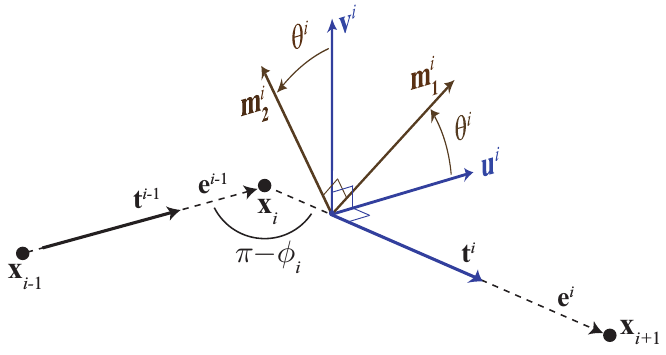
\includegraphics[width=0.5\textwidth]{img/rod_math_model}
    };
    \node at (3, -2) {
      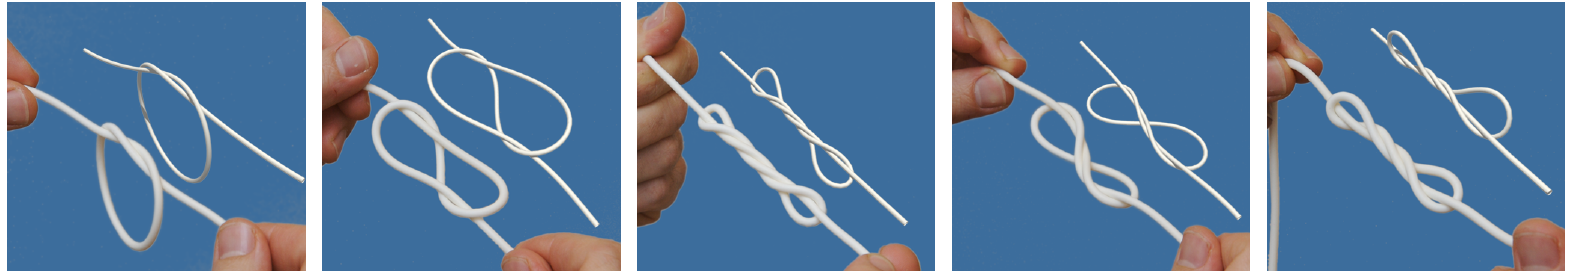
\includegraphics[width=0.6\textwidth]{img/real_rod}
    };
  }
\end{frame}

\begin{frame}
  \frametitle{Macroscopic Model}
  \begin{itemize}
  \item Anisotropic Kirchhoff plate
    \[
      W(\epsilon, \kappa) = \frac{1}{2}\epsilon :\mathbb{C}:\epsilon+\frac{1}{2}\kappa:\mathbb{B}:\kappa
    \]
  \item Strain-stress relationship
    \[
    \sigma = \mathbb{C}:\epsilon,\quad M = \mathbb{B}:\kappa
    \]
  \end{itemize}
\end{frame}

\begin{frame}
  \frametitle{Homogenization}
  \begin{itemize}
  \item Membrane material tensor fitting
    \[
    \mathbb{S}^H = \argmin_{\mathbb{S}} \sum_i^N \frac{1}{\|\epsilon_i\|_F^2}\|\mathbb{S}:\sigma_i-\epsilon_i\|_F^2
    \]
    \pause
  \item Data set construction
    \begin{itemize}
    \item[-] Generate deformation
    \item[-] Obtain macroscopic strain-stress pair
    \end{itemize}
  \end{itemize}
\end{frame}

\begin{frame}
  \frametitle{Homogenization}
  \begin{itemize}
  \item Generate deformation
    \begin{itemize}
    \item<1->[-] Uniaxial and biaxial stretch
    \item<2->[-] Periodical boundary condition
      \[x_j = x_i+d_{ij}\]
    \end{itemize}
  \item<3-> Calculate strain-stress pair
    \begin{itemize}
    \item<3->[-] Strain
      \[
      \begin{split}
        &F = [x_i-x_j, x_i-x_l][X_i-X_j, X_i-X_l]^{-1} \\
        &\epsilon = \frac{1}{2}(F^T+F)-I
      \end{split}
      \]
    \item<4->[-] Stress
      \[
      \sigma \cdot n = f \quad \Rightarrow \quad \sigma = [f_0, f_1][n_0, n_1]^{-1}
      \]
    \end{itemize}
  \end{itemize}
  \TikzDraw {
    \visible<1> {
      \node at (3.5, 1) {
        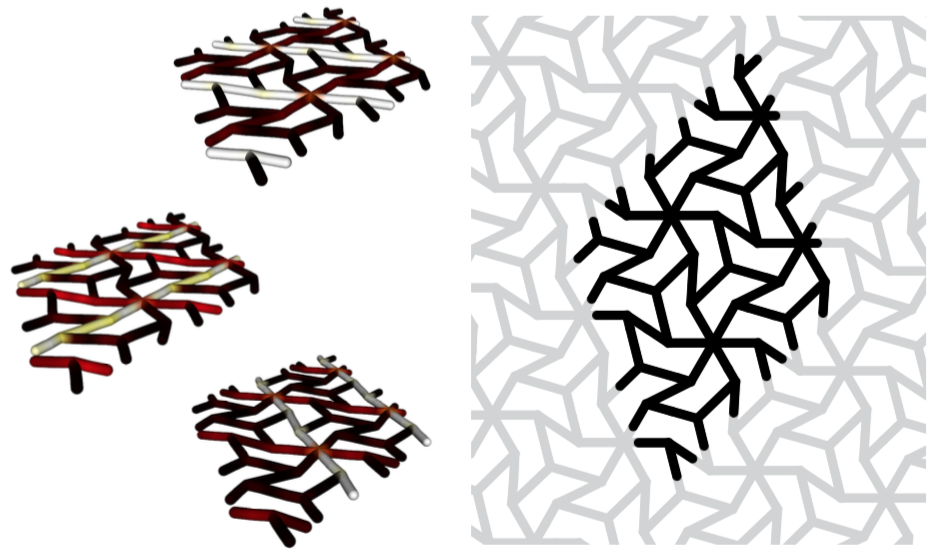
\includegraphics[width=0.4\textwidth]{img/membrane_defm}
      };
    }
    \visible<2> {
      \node at (4, 0) {
        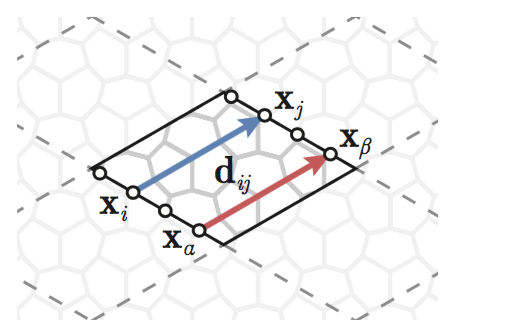
\includegraphics[width=0.3\textwidth]{img/membrane_bc}
      };
    }
    \visible<3-> {
      \node at (4, 1) {
        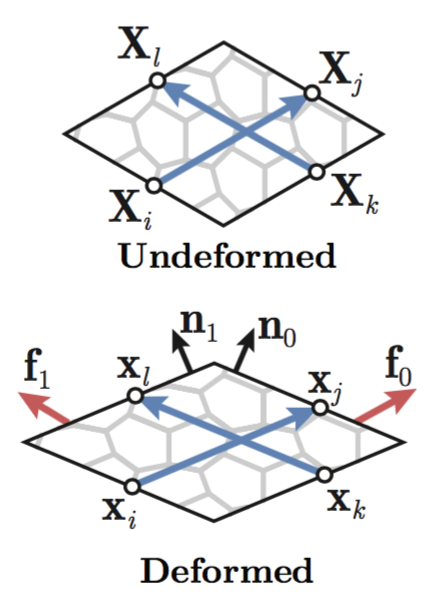
\includegraphics[width=0.2\textwidth]{img/strain-stress-calc}
      };
    }
  }
\end{frame}

\begin{frame}
  \frametitle{Homogenization}
  \begin{itemize}
  \item Bending material tensor fitting
    \[
    \mathbb{B}^H = \argmin_{\mathbb{B}}\sum_i^M (\frac{1}{2}\kappa_i:\mathbb{B}:\kappa_i-W_i)^2
    \]
  \item<2> Data set construction
  \end{itemize}
  \TikzDraw {
    \visible<3-> {
    \node at (-2.5, -2) {
      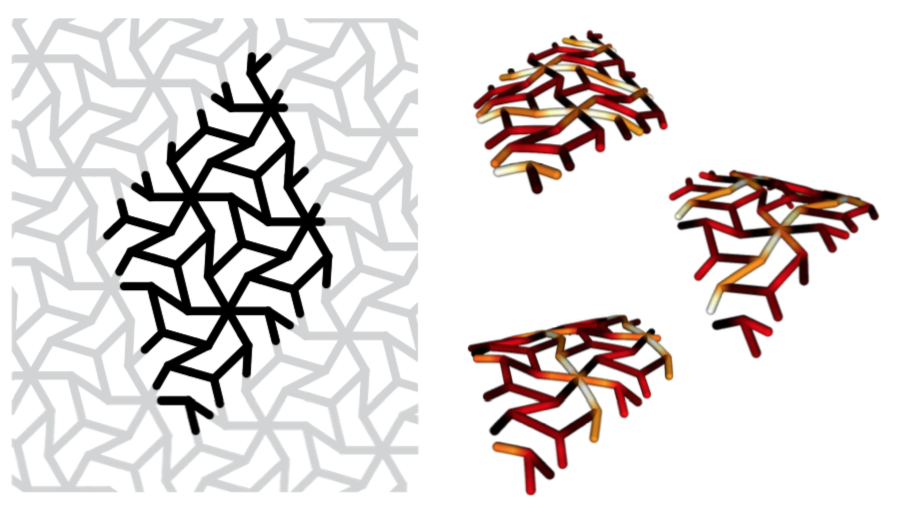
\includegraphics[width=0.5\textwidth]{img/bending_defm}
    };
    }
    \visible<4-> {
    \node at (3, -2) {
      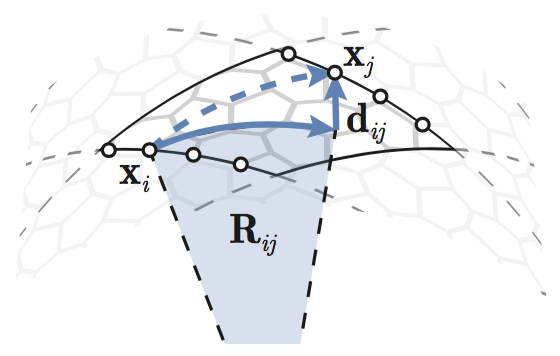
\includegraphics[width=0.5\textwidth]{img/bending_bc}
    };
    \node at (3, -4) {
      $\BOLD{x}_j = \BOLD{R}_{ij}\BOLD{x}_i+\BOLD{d}_{ij}$
    };
    }
  }
\end{frame}

\begin{frame}
  \frametitle{Homogenization}
  \begin{itemize}
  \item Determining the size of test set
    \begin{itemize}
    \item[-] Cross validation scheme.
    \end{itemize}
  \item Nonlinearities.
    \begin{itemize}
    \item[-] Multiple test sets with varying deformation magnitude
    \item[-] Uniaxial and biaxial deformation (0.1\% \& 10.0\%)
    \item[-] Curvature (0.1$m^{-1}$ \& 5$m^{-1}$)
    \end{itemize}
  \end{itemize}  
\end{frame}

\begin{frame}
  \frametitle{Investigate Direction-Dependent Elasticity}
  \begin{itemize}
  \item Young's modulus
    \[
    E(d) = \frac{1}{(dd^T):\mathbb{S}:(dd^T)}
    \]
  \item Poisson ratio
    \[
    \nu(d) = -\frac{(dd^T):\mathbb{S}:(nn^T)}{(dd^T):\mathbb{S}:(dd^T)}
    \]
  \item Bending stiffness
    \[
    b(d) = (dd^T):\mathbb{B}:(dd^T)
    \]
  \end{itemize}
\end{frame}

\begin{frame}
  \frametitle{Symmetries}
  \TikzDraw {
    \node at (-2.5, 0) {
      \parbox[t]{0.6\textwidth} {
        \begin{itemize}
        \item Geometric symmetries
          \begin{itemize}
          \item[-] Rotational symmetry
          \item[-] Reflection symmetry
          \end{itemize}
        \item Material symmetries
          \begin{itemize}
          \item[-] Anisotropic
          \item[-] Orthotropic
          \item[-] Tetragonal
          \item[-] Isotropic
          \end{itemize}
        \end{itemize}
      }      
    };
    \visible<2> {
      \node at (3, 0) {
        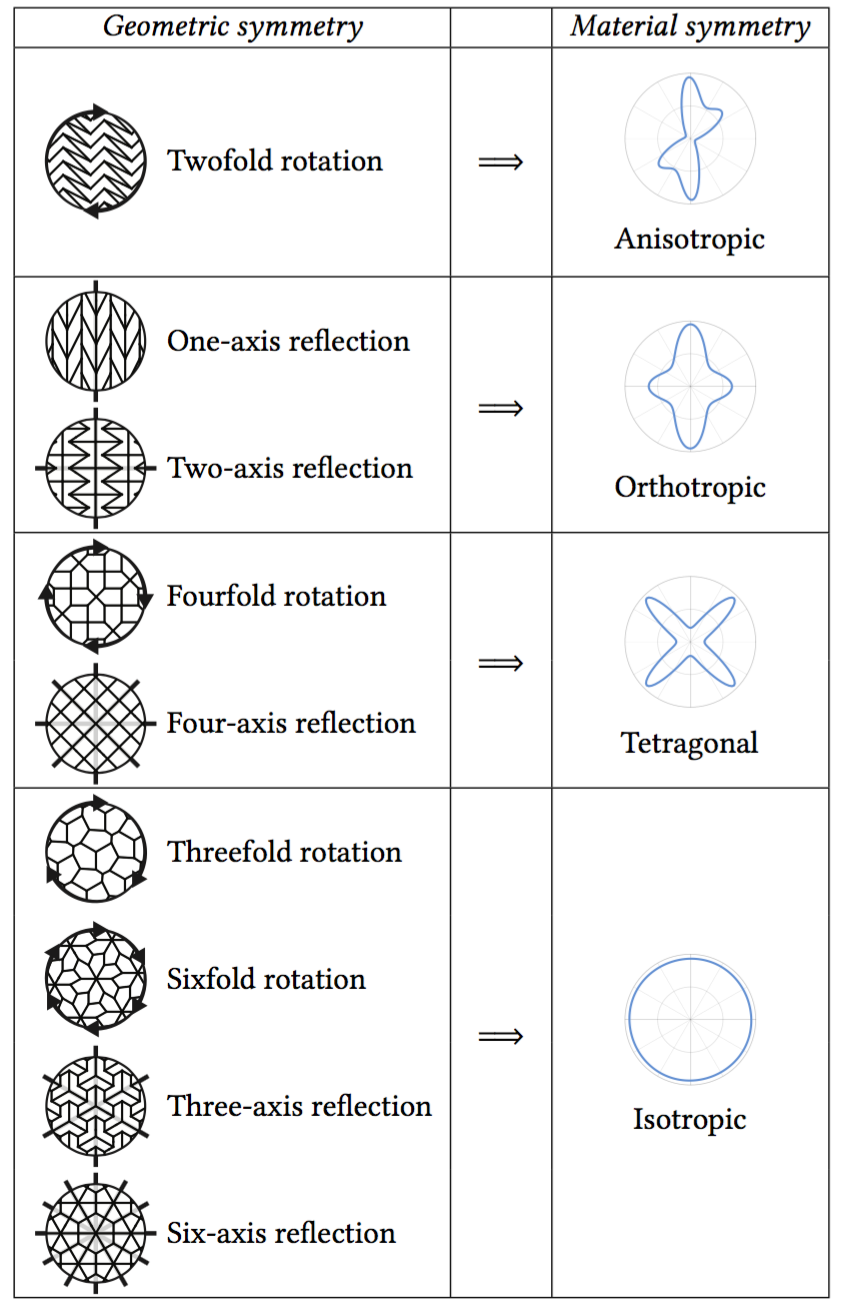
\includegraphics[width=0.5\textwidth]{img/symmetry}      
      };
    }
    \visible<3> {
      \node at (3, 0) {
        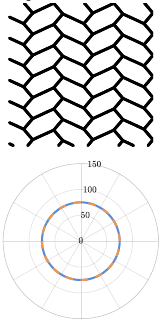
\includegraphics[width=0.3\textwidth]{img/inv_example}
      };
    }
  }
\end{frame}

\begin{frame} 
  \TikzDraw {
    \node at (0, 0.5) {\Huge{Experiments}};
  }
\end{frame}

\begin{frame}
  \frametitle{Validation}
  \TikzDraw{
    \node at (-3, 0) {
      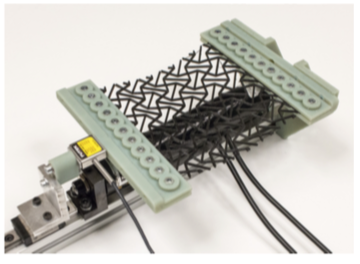
\includegraphics[width=0.4\textwidth]{img/real_mem_test}
    };
    \node at (3, 0) {
      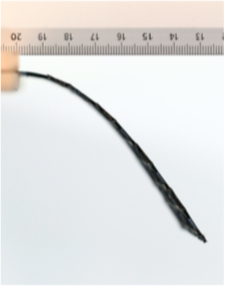
\includegraphics[width=0.3\textwidth]{img/real_bend_test}
    };
    \visible<2-> {
    \node at (0, 0) {
      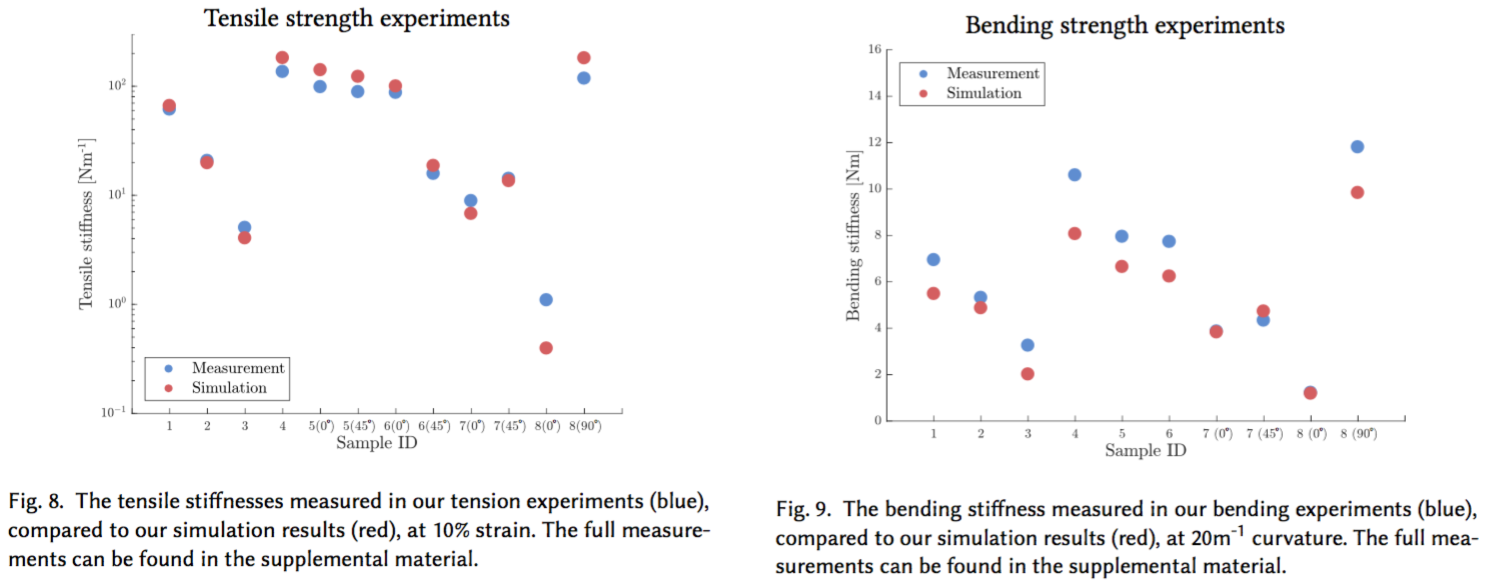
\includegraphics[width=\textwidth]{img/real_vs_sim}
    };
    }
  }
\end{frame}

\begin{frame}
  \frametitle{Isohedral Tilling Explorer}
  \begin{figure}
    \centering
    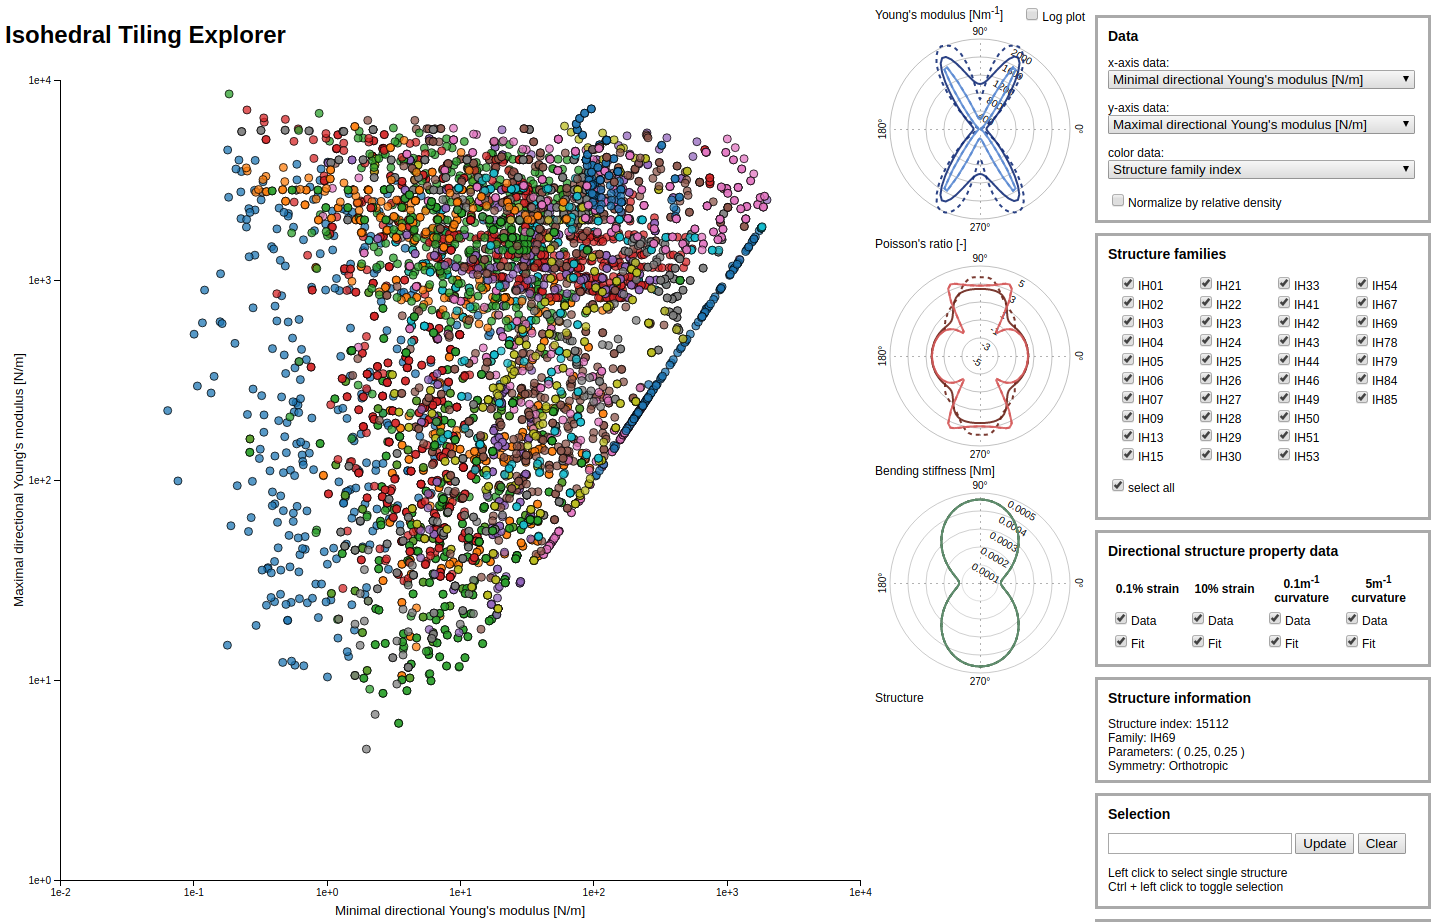
\includegraphics[width=\textwidth]{img/gallery}
  \end{figure}
\end{frame}

\begin{frame}
  \frametitle{Accuracy}
  \TikzDraw {
    \visible<1> {
      \node at (0, 0) {      
        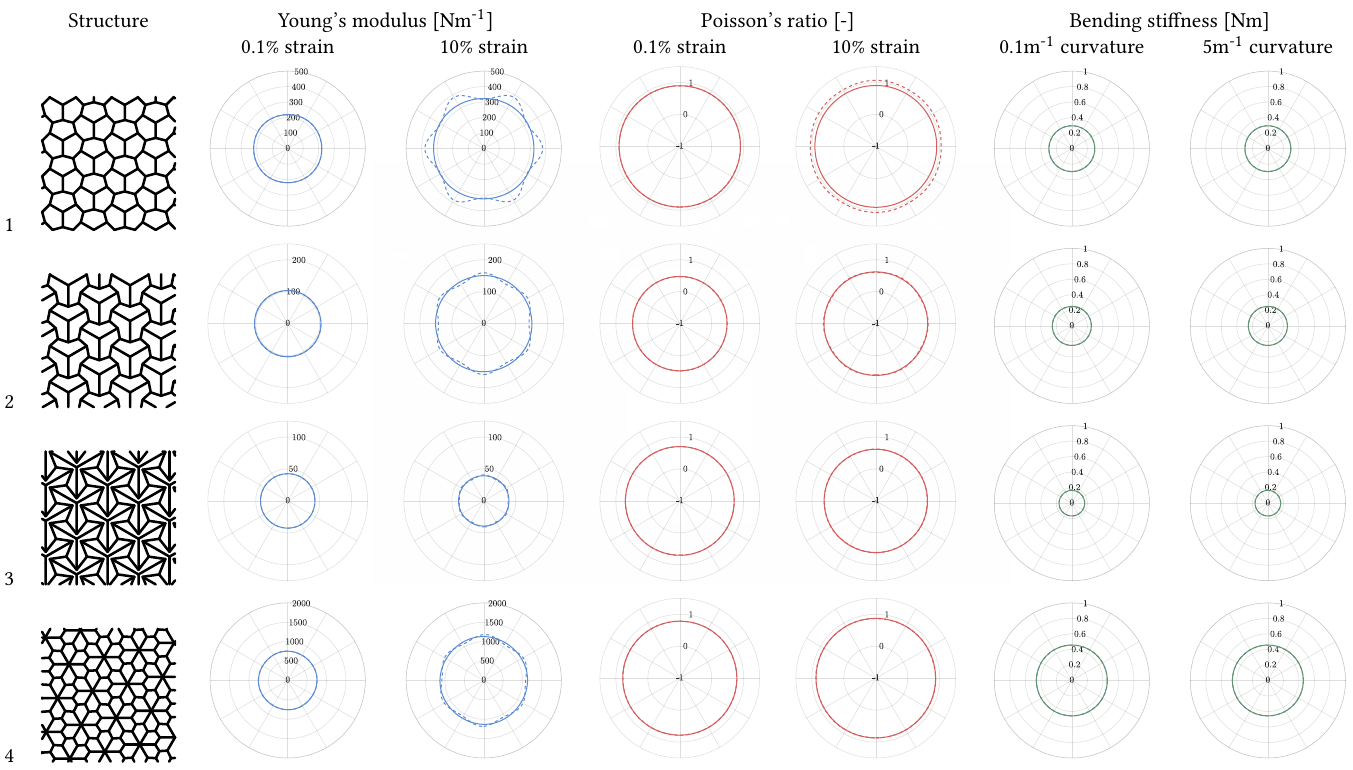
\includegraphics[width=\textwidth]{img/structure_group_1}
      };
    }
    \visible<2> {
      \node at (0, 0) {
        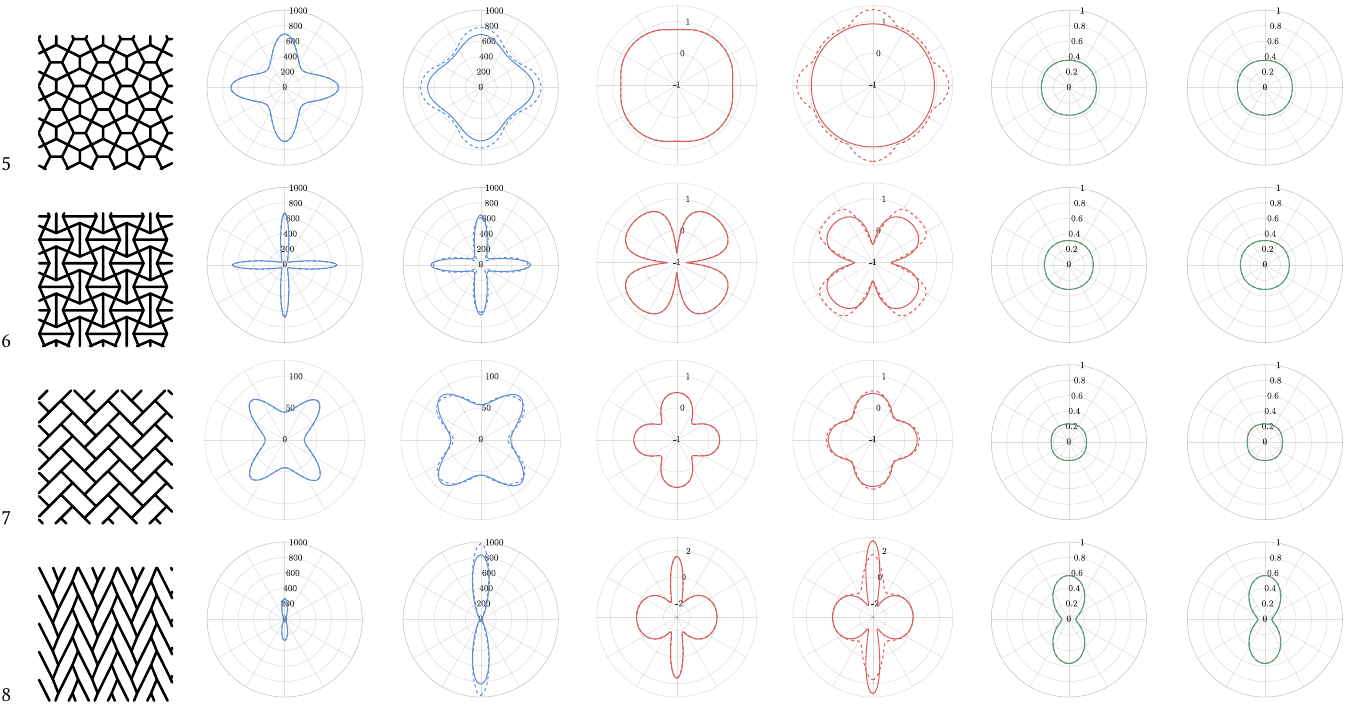
\includegraphics[width=\textwidth]{img/structure_group_2}
      };
    }
  }
\end{frame}


\begin{frame}
  \frametitle{Inverse structure optimization}
  \begin{figure}
    \centering
    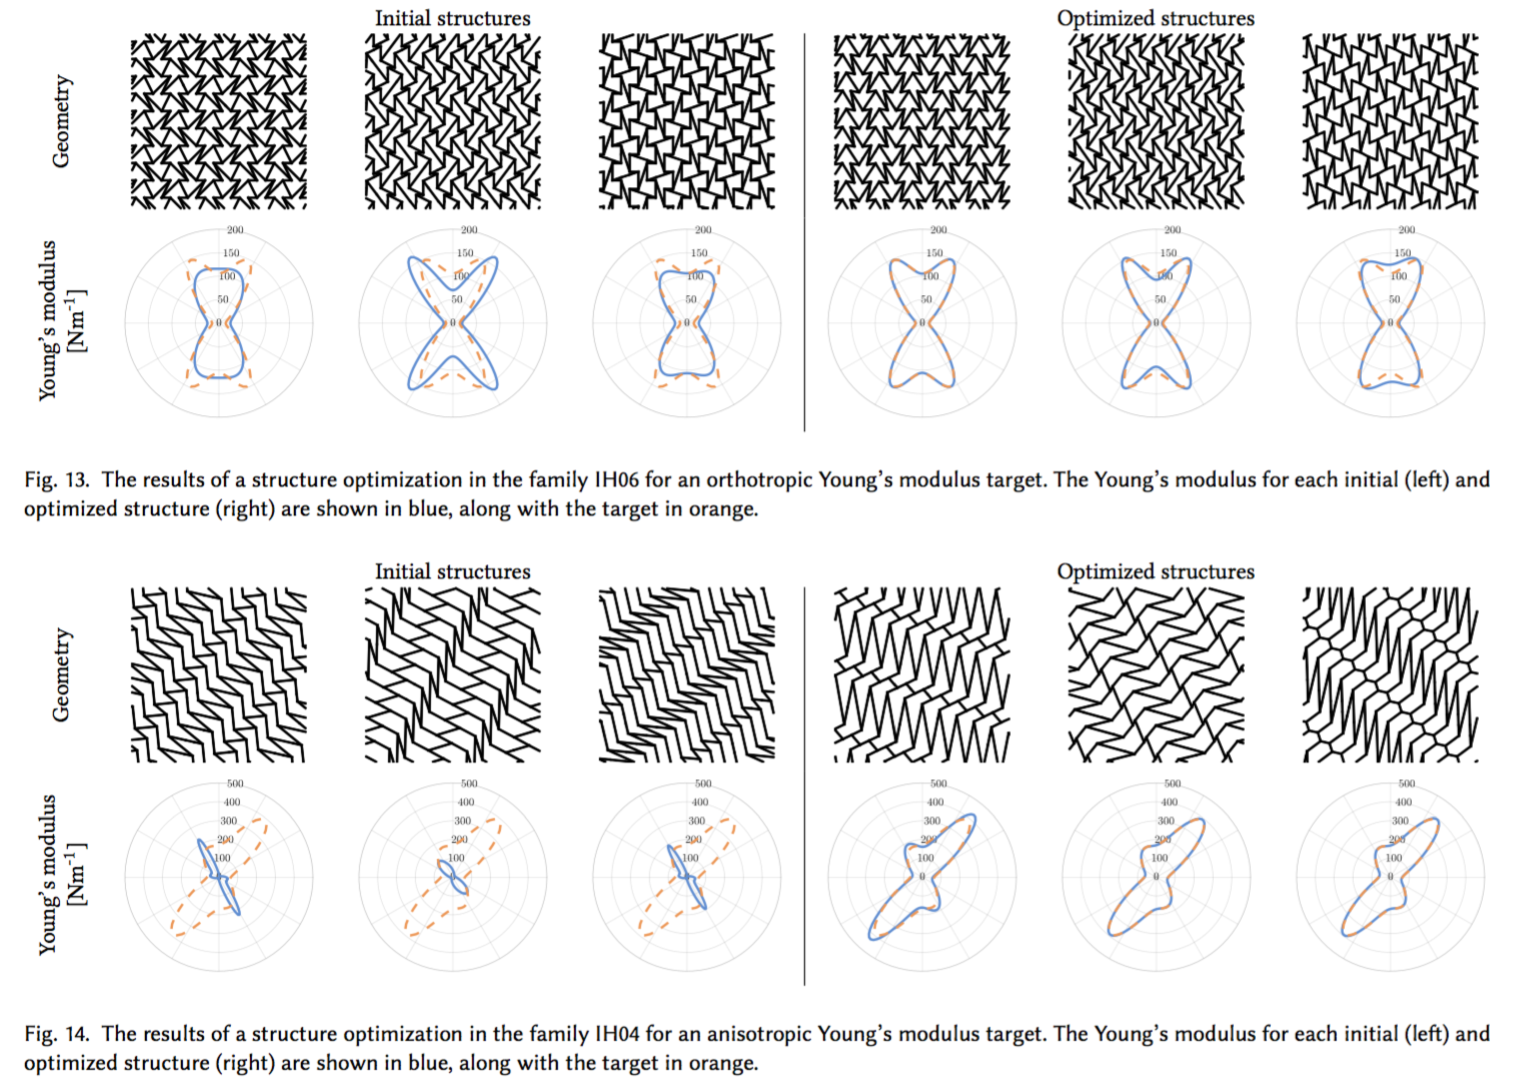
\includegraphics[width=\textwidth]{img/inv_opt}
  \end{figure}
\end{frame}

\begin{frame}
  \frametitle{Limitations and future work}
  \begin{itemize}
  \item Nonlinear macroscopic constitutive model.
  \item Characterization of irregular tillings.
  \end{itemize}
\end{frame}

\begin{frame} 
  \TikzDraw {
    \node at (0, 0.5) {\Huge{Thanks!}};
  }
  %\gridlines
\end{frame}

\end{document}
